\begin{frame}{Superposition von Neuronen}
\begin{columns}
		\alt<1>{\begin{column}{0.55\textwidth}
			\begin{itemize}
				\item{Neuronen: Bausteine des menschlichen Gehirns \textasciitilde $10^{11}$}
				\begin{itemize}
					\item{komplexes Netzwerk}
					\item{Verbindung mit dem Bewusstsein anzunehmen}
				\end{itemize}
				\item{Zwei mögliche Zustände}	
				\begin{itemize}
					\item{feuern $\leftrightarrow$ nicht feuern}
				\end{itemize}
			\end{itemize}
		\end{column}
		\begin{column}{0.4\textwidth}
			\centering
			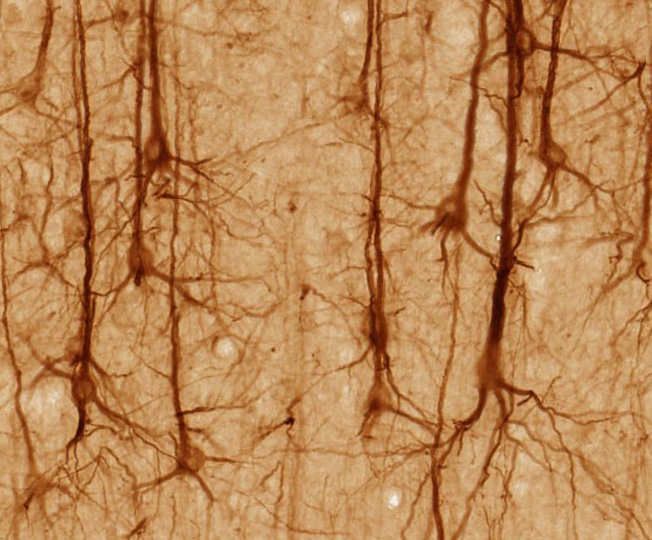
\includegraphics[scale=0.8]{graphics/neuron.jpg}\,\cite{neurons}
		\end{column}}{}
		\alt<2>{\begin{column}{0.45\textwidth}
			\begin{itemize}
				\item{Einfache Annahmen}
				\begin{beamerboxesrounded}{Anzahl der Na$^{\textcolor{white}{+}}$-Ionen}
					\begin{empheq}{equation*}
						N = \frac{\pi dLf\epsilon_{0}}{qh}\del{U_{1} -U_{0}}
					\end{empheq}
					\vspace{-0.5cm}
				\end{beamerboxesrounded}	

			\item{$h=\SI{8}{nm}$, $d=\SI{10}{\micro\metre}$,\\ $L=\SI{10}{\centi\metre}$, $f=\num{e-3}$,\\
				  $U_{0} = \SI{-0.07}{\volt}$, $U_{1} = \SI{0.03}{\volt}$}
				\begin{itemize}
					\item{$N \sim \num{e6}$}
				\end{itemize}
			\end{itemize}
		\end{column}
		\begin{column}{0.45\textwidth}
			\centering
			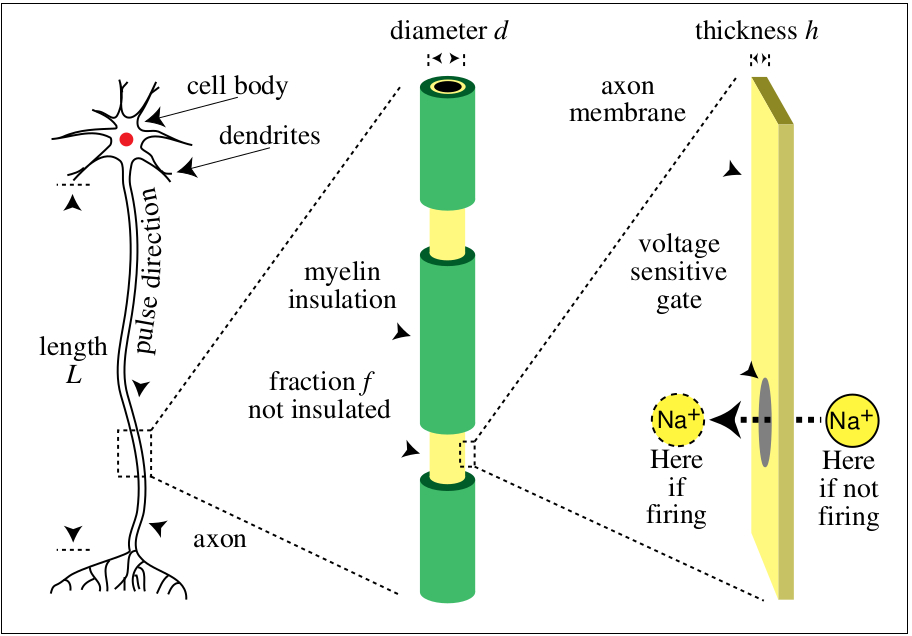
\includegraphics[scale=0.18]{graphics/neuron_schematic.jpg}\\\hfill\cite{Tegmark_99}
		\end{column}}{}
	\end{columns}	
	\alt<2>{\begin{itemize}
		\item[$\Rightarrow$]{Räumliche Superposition von \num{e6} Na$^{+}$-Ionen, mit Abstand  $\sim\mathcal{O}(\SI{10}{nm})$}
	\end{itemize}}{}
\end{frame}